\problemname{Talis' Fireball}

The battle had been raging for many rounds and your party is tired. Things are looking dark, until the wizard Talis realizes he has a 3rd level spell slot left.
That's enough for a Fireball! But while Talis is searching his scrolls, an arrow grazes his glasses. They fall to the ground and shatter into pieces. Now you all need to work together to find out how many people Talis can hit.
\\
\\
Your team will shout the amount of enemies and their coordinates to you. Then they will also shout their location, just so Talis doesn't hit them. Now it is up to you to find out how many enemies Talis can hit with one fireball. Once you tell him the max amount of enemies he can hit, Talis will use his wizard energy to feel where the fireball should hit on the battlefield.
\\
\\
In short, you need to calculate the maximum number of enemies Tails can hit with one Fireball.
\\
\\
Talis having no situational awareness states multiple rules for where he is willing to place the fireball and how big he can make it. While the rest of your party holds the enemies at bay.
\\
\\
All enemies, allies and the fireball itself will be placed on a grid, like shown in the picture. An enemy is considered hit by a fireball if the middle of the square is within the $2.5 m$ radius circle the fireball creates. The fireball cannot hit any ally, or Talis will refuse to throw it. Additionally, Talis can only throw the fireball so far, so we shall only consider an area of $450 m * 450 m$.

\begin{center}
  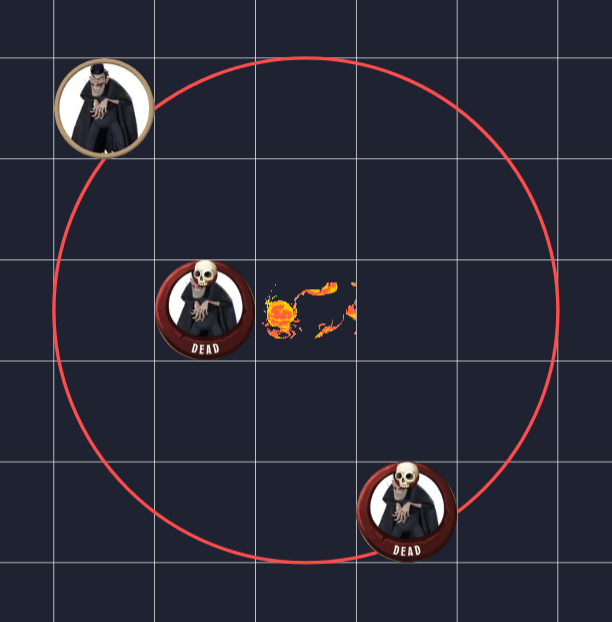
\includegraphics[width=0.5\textwidth]{Example.png}
\end{center}

\section*{Input}

The input consist of 4 lines. 
First line containing how many enemies there are on the battlefield $0 \leq e \leq 100000$\\
Second line contains e integers of coordinates of the enemies, seperated by spaces.\\
Third line contains how many party-members are on the battlefield $0 \leq f \leq 100000$ \\
Last line contains f integers of coordinates of your friends, seperated by spaces.

\section*{Output}

Output a single integer giving the maximum number of enemies a single fireball can hit at once, without hitting any friends. 
